\documentclass[]{article}
% used packages
\usepackage[german]{babel}   % enables umlaute
\usepackage[utf8]{inputenc}  % set encoding to utf8 otherwise no umlaute
\usepackage{graphicx}        % for including graphics
\usepackage{hyperref}        % for using hyperlinks in the document
\usepackage{tabularx}        % for extending tabluar
\usepackage{multirow}        % for rowspan in tabularx
\usepackage{ltablex}         % tables over multiple pages
\usepackage{textcmds}        % for quote support
\usepackage{pdfpages}        % for pdf include
\usepackage{caption}
\usepackage{minted}
\usepackage{listings}
\usepackage[left=1.0in, right=1.0in, top=1.0in, bottom=1.0in]{geometry} % for custom page layout

% Title Page
\title{Raspberry PI Security Application}
\author{Thonas Herzog, Philipp Wurm}


\newcommand{\imageDir}{images}
\newcommand{\dataDir}{data}
\newcommand{\dockerTestDir}{../java/testsuite/client/src/main/resources/docker}
\newcommand{\dockerRPIDir}{../host/docker}
\renewcommand\listingscaption{Quelltext}

\newenvironment{code}{\captionsetup{type=listing}}{}

\newmintedfile[yamlFile]{yaml}{
	linenos=true, 
	frame=single, 
	breaklines=true, 
	tabsize=2,
	numbersep=5pt,
	xleftmargin=10pt,
	baselinestretch=1,
	fontsize=\footnotesize
}
\newmintedfile[jsonfile]{json}{
	linenos=true, 
	frame=single, 
	breaklines=true, 
	tabsize=2,
	numbersep=5pt,
	xleftmargin=10pt,
	baselinestretch=1,
	fontsize=\footnotesize
}

\begin{document}
\maketitle

\section{Einleitung}
Dieses Dokument behandelt die Dokumentation des Projekts für die Lehrveranstaltung \emph{Service Engineering}, das eine Erweiterung des Projekts \emph{RPISec} für die Lehrveranstaltung \emph{Mobile und ubiquitäre Systeme} ist. Das Projekt \emph{RPISec} soll um einen OAuth2-Authentifizierungsservice erweitert werden und es sollen Integrationstests implementiert werden, welche die \emph{Microservice}-Infrastruktur mit \emph{Docker} testen.

\section{Entwicklungsrechner einrichten}
Dieser Abschnitt behandelt das Einrichten des Projekts \emph{RPISec} auf einem Entwicklungsrechner. Es werden Zugangsdaten für \emph{GMail}, \emph{Firebase} und \emph{Firebase Cloud Messasging} benötigt, die nicht in der Projektstruktur enthalten sind und extern verwaltet werden und daher eingebunden werden müssen.
{\renewcommand{\arraystretch}{2}%
\begin{center}
	\begin{tabular}{| c | l | p{7cm} |}
		\hline
		\textbf{Konfigurationsdatei} & \textbf{Beschreibung}  \\ \hline
		app.properties & Die externe Konfigurationsdatei für den Entwicklungsbetrieb für den \emph{App-Service} \\ \hline
		auth.properties & Die externe Konfigurationsdatei für den Entwicklungsbetrieb für den \emph{Auth-Service} \\ \hline
		app-test.properties & Die externe Konfigurationsdatei für die Integrationstests für den \emph{App-Service} \\ \hline
		auth-test.properties & Die externe Konfigurationsdatei für die Integrationstests für den \emph{Auth-Service} \\ \hline
		firebase-account.json & Die externe Konfigurationsdatei für die \emph{Firebase} Authentifizierung \\ \hline
	\end{tabular}
\end{center}
\ \newline
Diese Dateien sind im Verzeichnis \emph{$<doc\_location>/config$} enthalten, wobei die Datei \emph{firebase-account.json} und die \emph{GMail} Zugangsdaten ab 15.07.2016 18:00 nicht mehr gültig sein werden, da ab diesem Datum die Zugänge geschlossen werden.

\subsubsection{Auth-Service}
Mit folgenden \emph{Gradle} Befehl kann der \emph{Auth-Service} über die Kommandozeile gestartet werden. Um den Service in einer IDE zu starten kann eine \emph{Run Configuration} spezifisch für die IDE eingerichtet werden, die alle notwendigen \emph{Gradle} Kommandos und VM-Options definiert.
\begin{minted}{bash}
gradle buildFatJar bootRun
       -Dplatform=dev
       -Dadmin.email=<admin_email_address>                
       -Dspring.config.location=<fully_qualified_path_to_config_file>
\end{minted}
{\renewcommand{\arraystretch}{2}%
\begin{center}
	\begin{tabular}{| c | l | p{7cm} |}
		\hline
		\textbf{Parameter} & \textbf{Werte} & \textbf{Beschreibung}  \\ \hline
		platform & $dev$ & \textbf{dev}: Profil für die Entwicklung \\ \hline
		admin.email & Bsp.: admin@mail.com & Die Email-Adresse des Admins, der beim Start des Service erstellt wird. \\ \hline
		spring.config.location & Bsp.: /config.properties & Der voll qualifiziert Pfad zur externen Konfigurationsdatei  \\ \hline
	\end{tabular}
\end{center}

\subsubsection{App-Service}
Mit folgenden \emph{Gradle} Befehl kann der \emph{App-Service} über die Kommandozeile gestartet werden. Um den Service in einer IDE zu starten kann eine \emph{Run Configuration} spezifisch für die IDE eingerichtet werden, die alle notwendigen \emph{Gradle} Kommandos und VM-Options definiert.
\begin{minted}{bash}
gradle buildFatJar bootRun
	   -Dplatform=dev              
	   -Dspring.config.location=<fully_qualified_path_to_config_file>
\end{minted}
{\renewcommand{\arraystretch}{2}%
\begin{center}
	\begin{tabular}{| c | l | p{7cm} |}
		\hline
		\textbf{Parameter} & \textbf{Werte} & \textbf{Beschreibung}  \\ \hline
		platform & $dev$ & \textbf{dev}: Profil für die Entwicklung \\ \hline
		spring.config.location & Bsp.: /config.properties & Der voll qualifiziert Pfad zur externen Konfigurationsdatei  \\ \hline
	\end{tabular}
\end{center}

\subsubsection{Integrationstests}
Mit folgenden \emph{Gradle} Befehl können die Integrationstest über die Kommandozeile ausgeführt werden. Es muss sichergestellt werden, dass \emph{Docker} gestartet wurde und dass der Benutzer alle nötigen Rechte für \emph{Docker} hat. Auf einer \emph{Windows} Maschine muss sichergestellt werden, dass das Laufwerk wo die Quelltexte liegen als für \emph{Docker} freigegeben wurde. 
\begin{minted}{bash}
gradle cleanState clean perpareDockerInfrastructure test
       -Dplatform=integrationTest
       -Dapp.config=<fully_qualified_path_to_app_config_file> 
       -Dauth.config=<fully_qualified_path_to_app_config_file> 
       -DfirebaseConfig=<fully_qualified_path_to_firebase_json_file>
\end{minted}
{\renewcommand{\arraystretch}{2}%
\begin{center}
	\begin{tabular}{| c | l | p{7cm} |}
		\hline
		\textbf{Parameter} & \textbf{Werte} & \textbf{Beschreibung}  \\ \hline
		platform & $integrationTest$ & \textbf{dev}: Profil für die Integrationstests\\ \hline
		app.config & Bsp.: /app.properties & Der voll qualifiziert Pfad zur externen Konfigurationsdatei für den \emph{App-Service}  \\ \hline
		auth.config & Bsp.: /auth.properties & Der voll qualifiziert Pfad zur externen Konfigurationsdatei für den \emph{Auth-Service}  \\ \hline
		firebaseConfig & Bsp.: /app.properties & Der voll qualifiziert Pfad zur 
		\emph{firebase account} JSON Datei  \\ \hline
	\end{tabular}
\end{center}
In der Datei \emph{Gradle Build}-Datei \emph{java/testsuite/client/build.gradle} werden die beiden Umgebungsvariablen \emph{DOCKER\_COMPOSE\_LOCATION} und  \emph{DOCKER\_COMPOSE\_LOCATION} auf einem Windowssystem  automatisch gesetzt, wenn sie nicht vorhanden sind.

\section{OAuth2 Authentifizierungsservice}
Dieser Abschnitt behandelt die Dokumentation des OAuth2-Authentifizierungsservice, der für die Authentifizierung der mobilen \emph{Clients} für den bestehenden Applikationsservice sowie die Benutzerverwaltung verantwortlich ist. Der OAuth2-Authentifizierungsservice wurde mit \emph{Spring Boot} implementiert, wobei \emph{Spring Boot} schon alle benötigten Funktionalitäten für OAuth2 bereitstellt und die Applikation nur mehr konfiguriert werden muss.
\newline
\newline
\emph{Spring Boot} stellt ein Datenbankschema für OAuth2 zur Verfügung, was angewendet wurde und die OAuth2 \emph{Clients}, \emph{Tokens} usw. werden über JDBC in einer Datenbank verwaltet.
\newline
\newline
Neben diesen Datenbankschema wurden auch Benutzertabellen angelegt, die über JPA verwaltet werden und keine strikten Beziehungen zu OAuth2 Tabellen haben, jedoch halten die Benutzer die \emph{Id} des generierten Oauth2-Clients, damit sichergestellt werden kann, das bei Anfragen nur \emph{Client Credentials} akzeptiert werden, die auch dem Benutzer zugewiesen sind, was so in OAuth2 nicht vorgesehen ist.

\subsection{OAuth2 Authentifizierung}
Nachdem am Authentifizierungsservice mobile \emph{Clients} authentifiziert werden, wird für diese \emph{Clients} der OAuth2-\emph{Password Flow} verwendet. Da es vermieden werden soll diesen mobilen \emph{Clients} OAuth2-\emph{Client Credentials} mit auszuliefern, wird bei jedem \emph{Login} eines mobilen \emph{Clients} ein neuer \emph{OAuth2 Client} für diesen mobilen \emph{Client}  angelegt und gegebenenfalls ein bereits existierender gelöscht, damit werden bei jedem Login neue \emph{Client Credentials} für die mobilen \emph{Clients} generiert.
\newline
\newline
OAuth2 würde jede gültigen Zugangsdaten für jeden existierenden OAuth2-\emph{Client} akzeptieren, was so geändert wurde, dass nur Zugangsdaten von Benutzer akzeptiert werden, die dem OAuth2-\emph{Clients} zugewiesen sind. Dadurch sind die OAuth2-\emph{Clients} Benutzer direkt zugeordnet und können nicht von anderen Benutzern verwendet werden, was meiner Meinung nach die Sicherheit erhöht.

\subsection{Benutzerverwaltung}
Dieser Abschnitt der Dokumentation behandelt die Benutzerverwaltung, die Teil des Authentifizierungsservice ist. Da es sich um eine Sicherheitsanwendung handelt wollen wir keine Benutzerverwaltung von anderen Services nutzen, sondern wollen die Benutzer selbst verwalten, was im Authentifizierungsservice implementiert wurde. Es wurden JPA-\emph{Entitäten} \emph{User} und \emph{ClientDevice} implementiert, wobei \emph{ClientDevice} die Referenz auf den erstellten OAuth2-\emph{Clients} für den Benutzer hält.
\newpage

\subsubsection{\emph{Client} Login}
\begin{figure}[h]
	\centering
	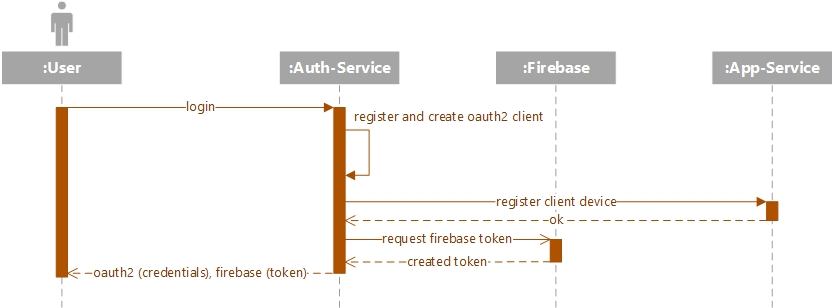
\includegraphics[scale=0.75]{\imageDir/sequence-client-login-auth-only.jpg}
	\caption{Sequenzdiagramm des Logins über einen mobilen \emph{Client}}
	\label{fig:image-sequence-client-login}
\end{figure}
\ \newline
Die Abbildung \ref{fig:image-sequence-client-login} zeigt den Ablauf des Logins eines Benutzers über einen mobilen \emph{Client}. Der Benutzer wird mit seinen Zugangsdaten via REST am Authentifizierungsservice authentifiziert und es wird ein OAuth2-\emph{Client} für das verwendete Endgerät erstellt, wobei die \emph{Client}-Anwendung einen eindeutigen Schlüssel für jedes Endgerät erzeugen muss. Dieser registrierte \emph{Client} wird an den Applikationsservice via REST übermittelt. Anschließend wird für den \emph{Client} auf \emph{Firebase} ein Token erstellt, mit dem sicher der \emph{Client} auf \emph{Firebase} authentifizieren kann. Als Antwort wird dem \emph{Client} folgendes JSON-Resultat übermittelt.
\newline
\begin{code}
	\caption{JSON-Antwort an den \emph{Client}}
	\jsonfile{\dataDir/client-login-json-response.json}
\end{code}
\ \newline
Das Registrieren des Clients am Applikationsservice erfolgt über Basic Authentifizierung geschützte Schnittstelle, die nur für einen Systembenutzer nutzbar ist, der dem Authentifizierungsservice bekannt ist.

\subsubsection{\emph{Client} \emph{Firebase Cloud Messaging Token (FCM)} Registrierung}
Die Abbildung \ref{fig:image-sequence-fcm-token-registration} zeigt den Ablauf der Registrierung des FCM-Tokens am Applikationsservice über den Authentifizierungsservice. Die Registrierung über den Authentifizierungsservice wurde gewählt, da dieser Service die Benutzer und deren Endgeräte verwaltet. Das Registrieren des FCM-Tokens am Applikationsservice erfolgt über Basic Authentifizierung geschützte Schnittstelle, die nur für einen Systembenutzer nutzbar ist, der dem Authentifizierungsservice bekannt ist. 
\newpage
\begin{figure}[h]
	\centering
	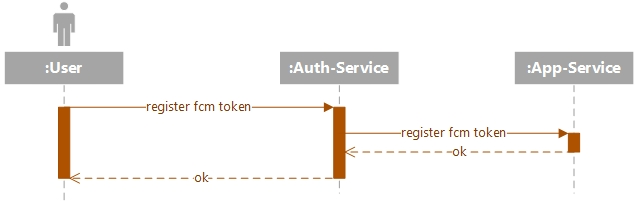
\includegraphics[scale=0.75]{\imageDir/fcm-token-registration}
	\caption{Sequenzdiagramm der Registrierung des FCM-Token}
	\label{fig:image-sequence-fcm-token-registration}
\end{figure}
\ \newline
Als Resultat wird bei dieser Schnittstelle nur der Http Statuscode 200 zurückgeliefert.

\subsection{\emph{Swagger Client} Generierung}
\label{sec:swagger-client-generation}
Dieser Abschnitt behandelt die Generierung der \emph{Client-API} mit \emph{Swagger}. Das \emph{OpenSource}-Projekt \emph{SpringFox} stellt eine Integration von \emph{Swagger} für \emph{Spring MVC} zur Verfügung mit der aus \emph{RestController} \emph{Swagger}-Definitionen erstellt werden können. Des Weiteren wird die \emph{Swagger-UI} mitgeliefert, mit der die implementierten REST-Schnittstellen getestet werden können.
\newline
\newline
Aus den generierten \emph{Swagger}-Definition der \emph{Microservice} spezifischen REST-Schnittstellen wurden \emph{gradle} Projekte generiert, welche die \emph{Client} Implementierungen enthalten. Die generierten Projekte wurden in das Wurzelprojekt \emph{java} aufgenommen, in dem alle Projekte des Projekts \emph{RPISec} enthalten sind.
\newline
\newline
Für die Generierung wurden die beiden Skripte \emph{generate-clients.bat} und \emph{update-clients.bat} implementiert, wobei das Skript \emph{generate-clients.bat} die Projekte und \emph{Client} Implementierungen generiert und das Skript \emph{update-clients.bat} nur die \emph{Client} Implementierungen generiert. Damit die \emph{Client} Implementierungen generiert werden können, müssen die Services gestartet sein.
\newline
\newline
Die \emph{Swagger-UI} kann unter folgenden Link erreicht werden \emph{$<BASE\_URL>$/swagger-ui.html}, wobei die \emph{BASE\_URL} der Pfad ist, unter dem der \emph{Microservice} erreicht werden kann. Die \emph{BASE\_URL} hat das Format \emph{$<PROTOCOL>$://$<HOST>$:$<PORT>$/$<CONTEXT\_ROOT>$/}. 
\newpage

\section{Integrationstests}
Dieser Abschnitt behandelt die Integrationstests für die implementierten \emph{Microservices} in einer Docker Infrastruktur.
\begin{figure}[h]
	\centering
	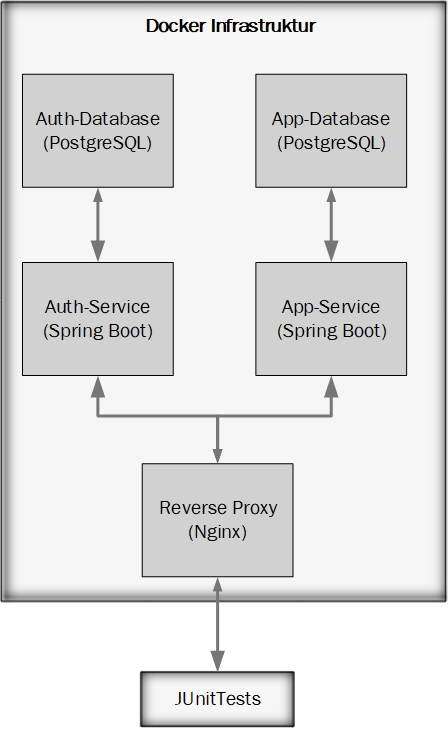
\includegraphics[scale=0.55]{\imageDir/integration-tests-docker-infrastructure}
	\caption{Aufbau der Integrationstests mit Docker Infrastruktur}
	\label{fig:integration-tests-docker-infrastructure}
\end{figure}
\ \newline
Die Abbildung \ref{fig:integration-tests-docker-infrastructure} zeigt den Aufbau der Docker Infrastruktur und die Verbindung zu den implementierten JUnit-Tests. Die Tests wurden in einer Suite zusammengefasst, wobei diese Suite eine \emph{Junit ClasRule} definiert, welche die Docker Infrastruktur via \emph{Docker Compose} vor der Ausführung der \emph{Suite} erstellt und startet und nach er Ausführung der \emph{Suite} die Infrastruktur stoppt und die \emph{Docker Container} entfernt. Die gesamte Infrastruktur ist aufgebaut, wie sie auch im produktiven Betrieb genutzt wird, jedoch konnten die \emph{Dockerfiles} nicht wiederverwendet werden, da dort ARM basierende \emph{Base Images} verwendet werden und die Tests auf einer x86 Architektur ausgeführt werden. Sie sind aber gleich nur das die \emph{Dockerfiles} der Tests von \emph{Base Images} ableiten, die auf einer x86 Architektur aufbauen.
\newline
\newline
Da ein eigenes \emph{Base Image} verwendet wird muss dieses \emph{Image} bevor die Tests ausgeführt werden mit folgenden Befehl erstellt werden. Dazu muss vorherig in das Verzeichnis \emph{testsuite/client/src/main/resources/docker} gewechselt werden.
\begin{minted}{bash}
docker build -t rpisec-test-base base/.
\end{minted}
Als Implementierung der \emph{JUnit ClassRule} wird die Bibliothek \emph{docker-compose-rule-junit4}\footnote{\url{https://github.com/palantir/docker-compose-rule}} von \emph{Palantir} verwendet, die es erlaubt über einen \emph{Builder} die \emph{ClassRule} zu konfigurieren und zu erstellen. Jedoch hat sich gezeigt, dass wenn während der Ausführung eine Ausnahme ausgelöst wird, die \emph{Docker Infrastruktur} nicht richtig runter gefahren wird und dadurch \emph{Docker Container} Namenskonflikte auftreten, die ein erneutes Starten der Tests verhindern.
\newline
\newline
Die Tests nutzen die in Abschnitt \ref{sec:swagger-client-generation} beschriebenen generierten \emph{Swagger Clients}, um die Kommunikation der \emph{Clients} mit den \emph{Microservices} und der Kommunikation der \emph{Microservices} untereinander zu testen. Es sei aber angemerkt das es sich hier um reine \emph{Blackbox} Tests handelt, die nur aus der Sicht der \emph{Clients} testen.
\end{document}           
